% !TEX root = main.tex

\chapter{Experimental results}
This chapter collects all the experimental results obtained during the thesis. Apart from the AOD characterization, there are two main sections. The first one contains the measurements carried out on the test setup done to asses the performance of the system. Here, polarization, stability, and focus spot has been checked. In particular, two methods have been used to measure $\mu$m focus spot: razor blade scans, and small pixel size camera. The other section comprises more advanced quantum optic experiments realized with ions and the final installed system. Ramsey spectroscopy was used to check addressing error and focus spot. Moreover, photons have been generated from one single ion with adjacent unperturbed ions.

\section{AOD}
The AOD is the core element of the setup, it is therefore essential to characterize it. The two main parameters we are interested in are the diffraction efficiency and the response time. For the diffraction efficiency we measure the total output power of the light $P_{tot}$ and then the power of the first diffracted order $P_{1}$. Diffraction efficiency is defined as the ratio between the two.
\begin{equation}
\text{DE} = \frac{P_1}{P_{tot}}.
\end{equation}
Before measuring the diffraction, the optimal RF power to drive the AOD has been found. This was done by measuring the power at the central frequency of the AOD and maximizing the light in the first diffracted order. Power measurements of the light were done with a Thorlabs PM100D, and the AOD was driven with a signal generator. The optimal RF power was found to be 0.11 W, and for the rest of the measurements it was kept as that value. Furthermore, the input polarization was optimized with a half wave plate, always trying to maximize the power of the diffracted light. In figure \ref{DE} the plot of the diffraction efficiency as a function of the RF frequency is displayed. Within a bandwidth of 50 MHz from 105 MHz to 155 MHz, we can see that more than 70 \% of the light is in the first diffracted order as expected from the datasheet, even though the bandwidth looks shifted with respected to the nominal central frequency of 120 MHz.\\
The response time is the time that it takes for the light to move when the RF frequency is changed. In order to perform this measurement, a voltage controlled oscillator (VCO) was used to generate the RF signal. The VCO was supplied a square wave that jumped between two voltages corresponding to two different frequencies. The blue light was measured with a photodiode. The photodiode was aligned with the light at one particular frequency, such that when the light moves, the beam would not hit the chip and the signal generated changes. In figure \ref{response}, the signal of the photodiode, together with the supplied VCO signal are plotted. Response time is $\sim 7-8\,\mu$s, in this time the light completely move from one angle to another one.

\begin{figure}
\centering
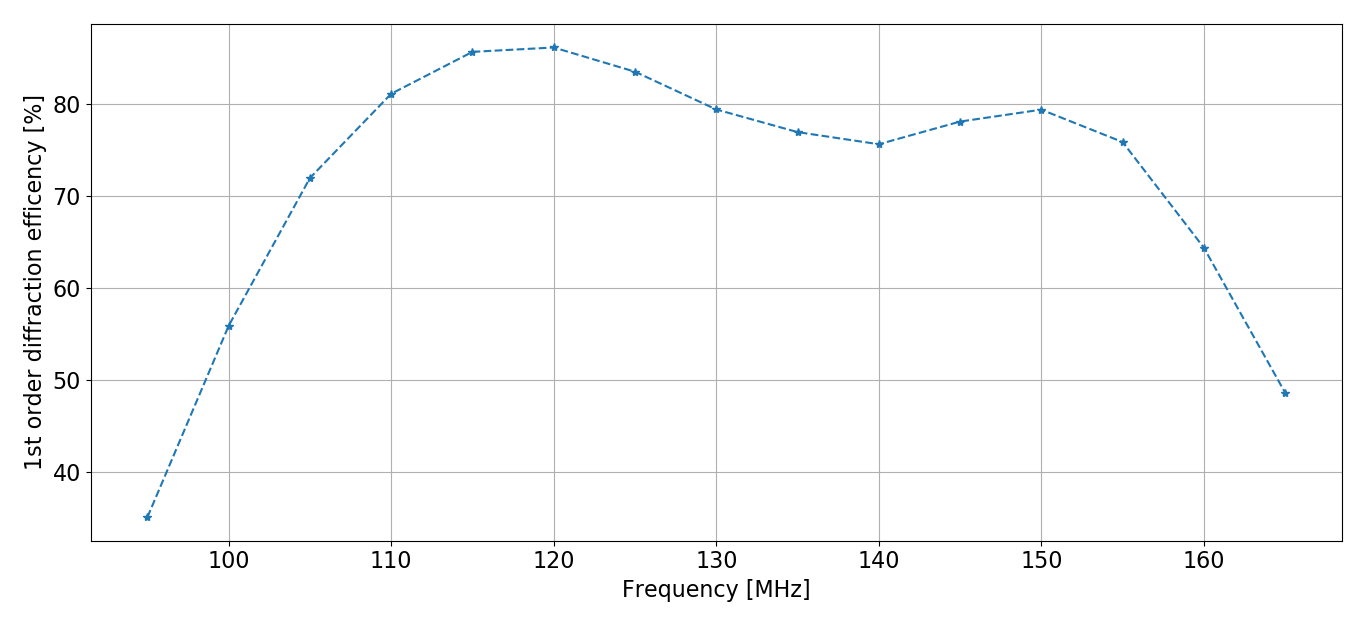
\includegraphics[width = .95\textwidth]{DE}
\caption{Diffraction efficiency of the AOD as a function of the RF driving frequency.}
\label{DE}
\end{figure}

\begin{figure}
\centering
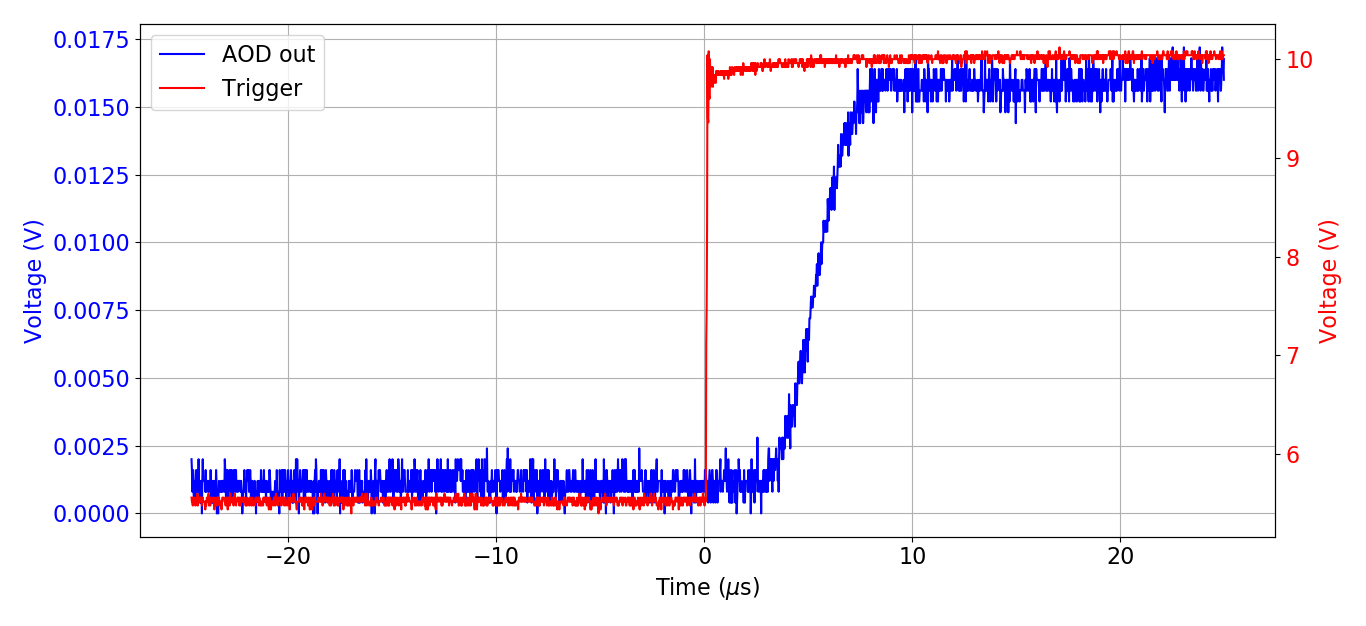
\includegraphics[width = .95\textwidth]{response}
\caption{Response time of the AOD, plotted are the photodiode signal in blue on the left $y$ axis, and the VCO voltage is in red on the right axis.}
\label{response}
\end{figure}

\section{Full test setup characterization}
The test setup was built on a spare optical table with a spare objective. The layout of the setup was as close as possible to the final version, so the system in figure \ref{addressingsetup} was replicated. The most important assessment was the focus spot, i.e. we tried to measure the waist of the beam and check if it was within requirements.
This is measured in two different ways: first we used a technique called Knife-edge, where the beam is scanned with a razor blade; then we also tried to measure it directly with a camera equipped with 1.6 $\mu$m pixel size.\\
Other than the waist size, we also measured stability of the system and the polarization capabilities.

\subsection{Waist: Knife-Edge method}
\begin{figure}[H]
\centering
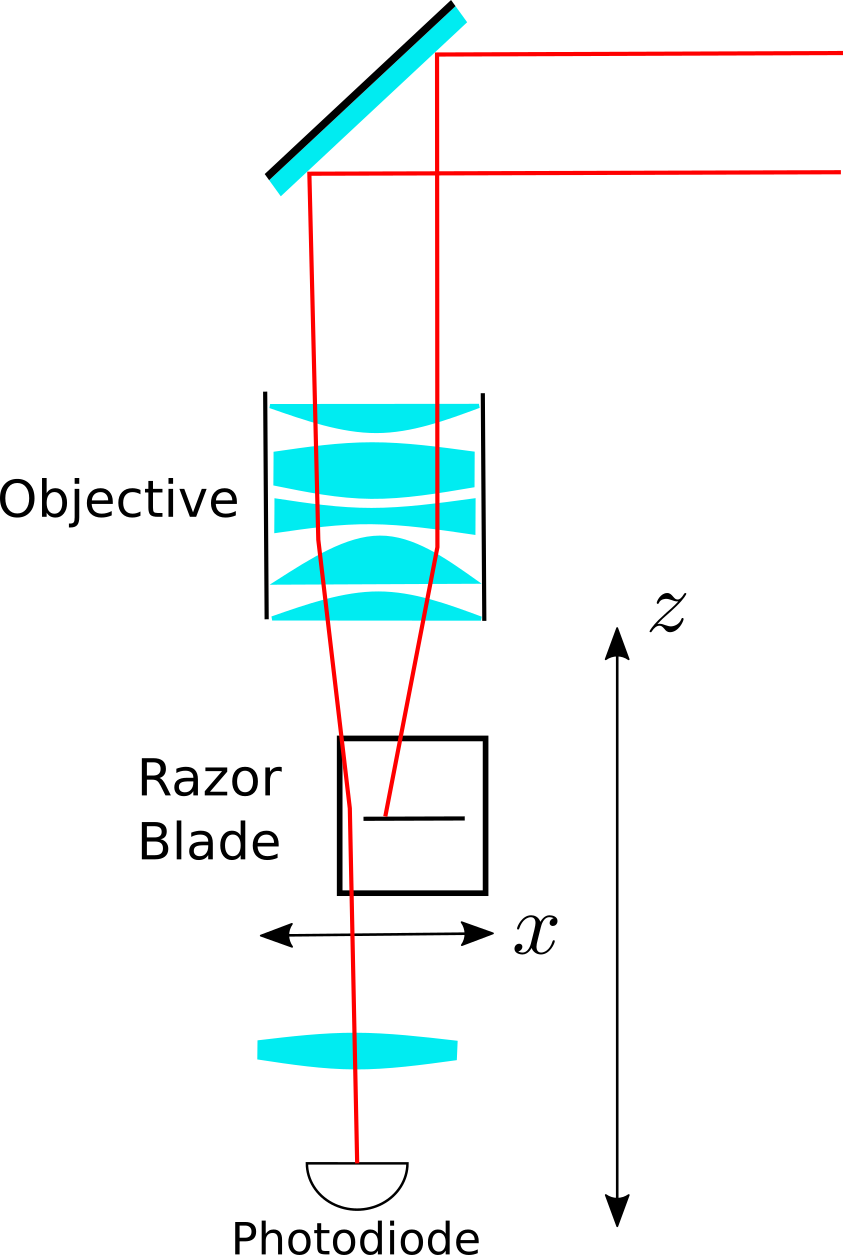
\includegraphics[width=.4\textwidth]{razorsetup}
\caption{Scheme of the razor scan.}
\label{razorscan}
\end{figure}
Measuring a micrometer waist is not easy task, the first approach we tried consists of mounting a razor blade on a translational stage. The stage is then moved in the $x$ direction cutting the beam perpendicularly such that the blade is scanning the beam profile. The setup used is showed in figure \ref{razorscan}, after the objective the blade is present, and since the beam is quickly diverging after the focus, a lens is used to refocus the light into a photodiode. A filter was also inserted in order to not saturate the photodiode.
The stage had to be moved with sub-micrometer precision, so the screw was a piezo actuator controlled by custom software. The same software also controlled a multimeter that measured the voltage of the photodiode. To get the whole profile of the beam, i.e. $W(z)$, the measurement procedure was as follow
\begin{itemize}
\item Position blade at appropriate $z$ coordinate
\item Scanning beam in $x$ direction with blade
\item Beam width extrapolation
\item Shift $z$ direction
\end{itemize}
And the procedure is repeated for sufficient values of $z$ to scan at least few Raylegh ranges. The beam width can be calculated from the scans by fitting of the data with \cite{knifeedge}
\begin{equation}
P(x,z) = \frac{P_0}{2}\text{erfc}\left[\frac{\sqrt{2}(x-x_0)}{W(z)} \right].
\end{equation}
Where the fitting parameters are $P_0, x_0,$ and the width $W(z)$. An example of scan is in figure \ref{examplerazorscan}. The errorbars comes from statistical average, every data point is a mean over 5 measurement, and the error is the standard deviation. The fit in this case gave a width of $3.47\pm 0.06\,\mu$m, the smallest width obtained with this method. Unfortunately, it is broader that the initial expectations. A possible explanation is that this method is not suitable for measuring micrometer waists with a razor blade, the roughness of the surface could limit the result. In comparison, authors of \cite{Cannon:86} have used, instead of a common razor blade, a glass substrate etched with an effective knife-edge feature.


\begin{figure}
\centering
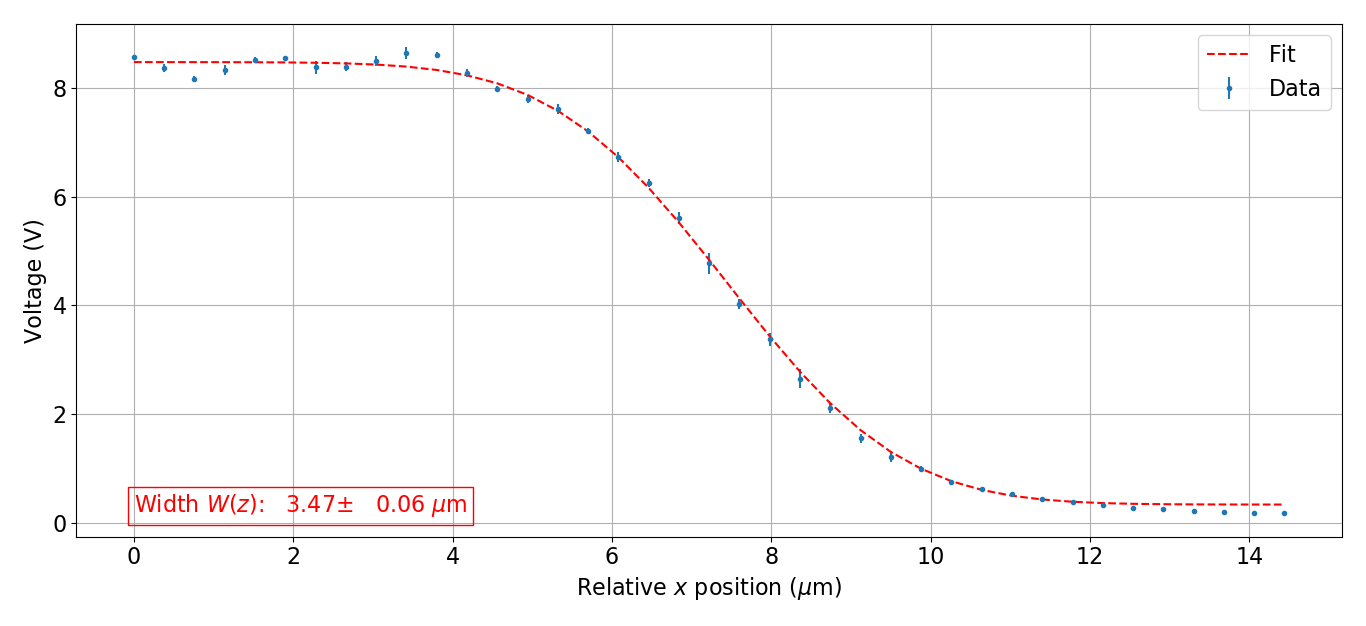
\includegraphics[width=1\textwidth]{img/razorscan}
\caption{Example of razor scan}
\label{examplerazorscan}
\end{figure}
\subsection{Waist: Camera}


\begin{figure}[H]
\centering
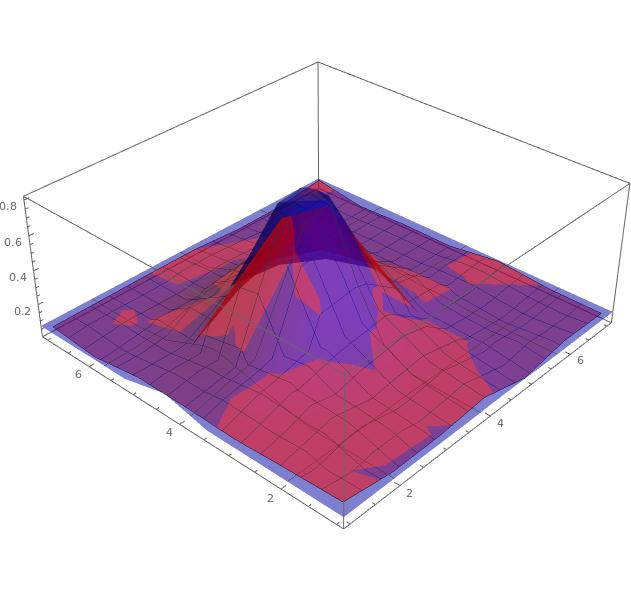
\includegraphics[width=\textwidth]{img/camera}
\caption{Example of camera picture}
\end{figure}
\subsection{Polarization characterization}
\subsection{Stability}
\section{Final installed system}
\subsection{Ramsey interferometry}
\begin{figure}[H]
\centering
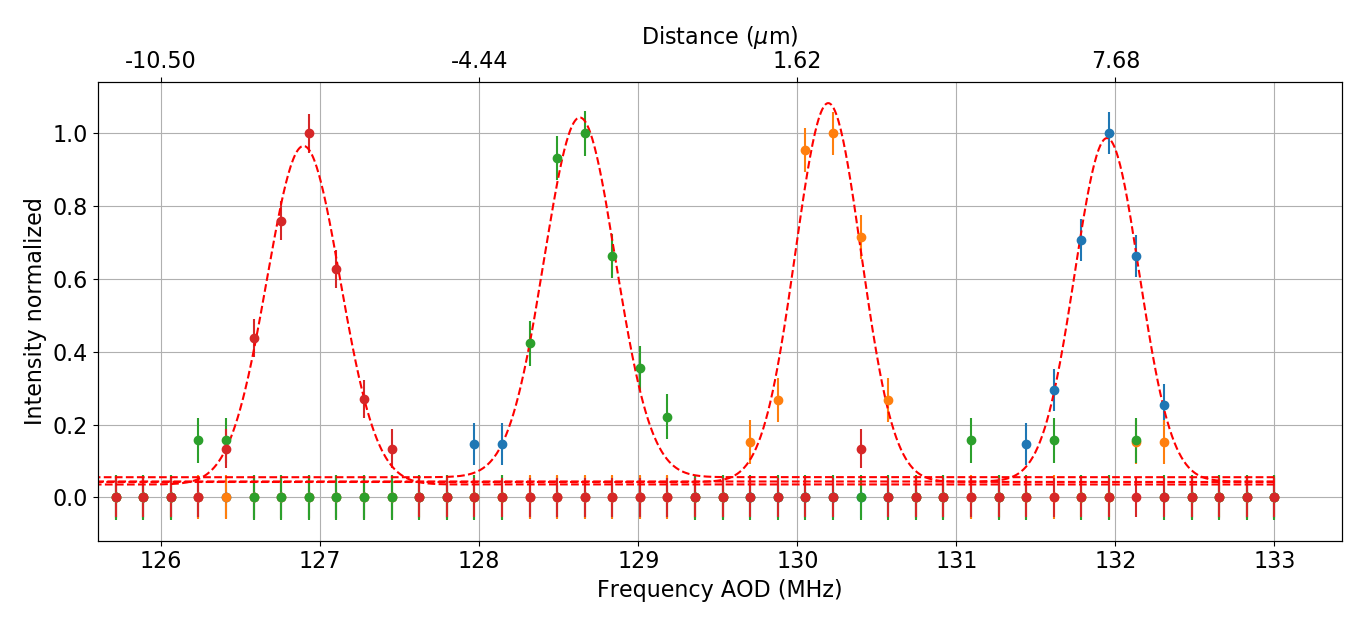
\includegraphics[width=\textwidth]{img/AODscan}
\caption{3 ions scanned}
\end{figure}
\begin{figure}[H]
\centering
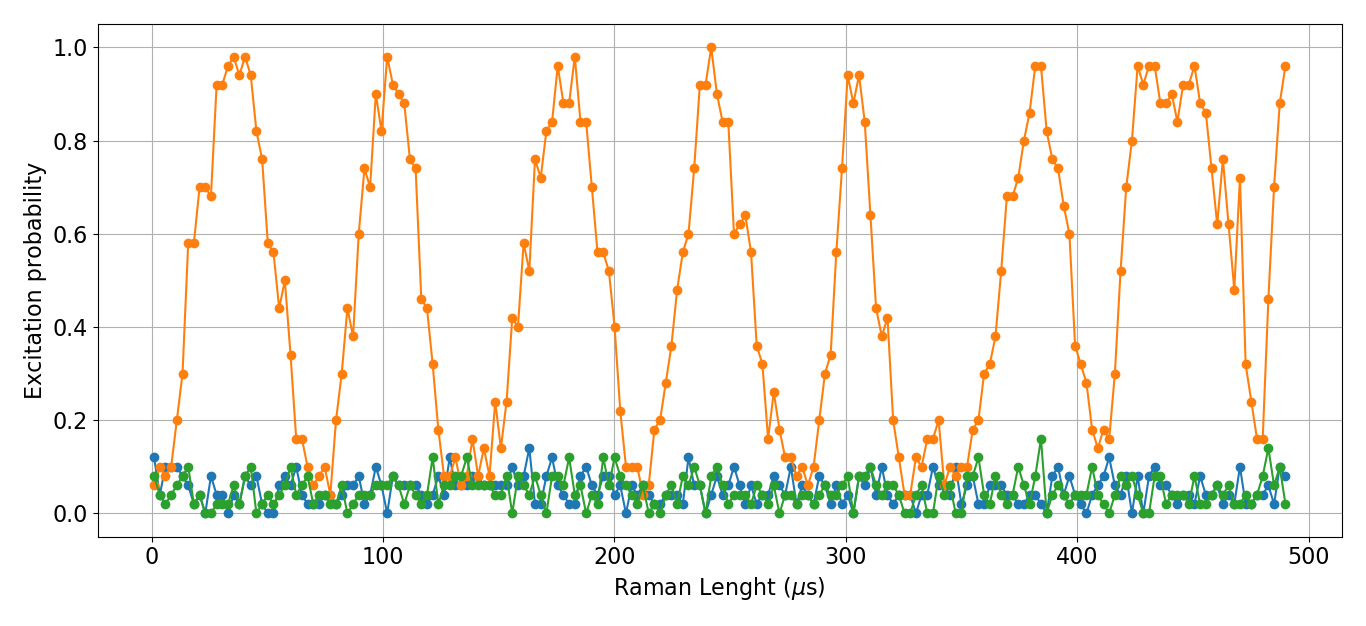
\includegraphics[width=\textwidth]{img/ac_stark}
\caption{393nm AC-Stark flops}
\end{figure}

\subsection{Photons production}
\begin{figure}[H]
\centering
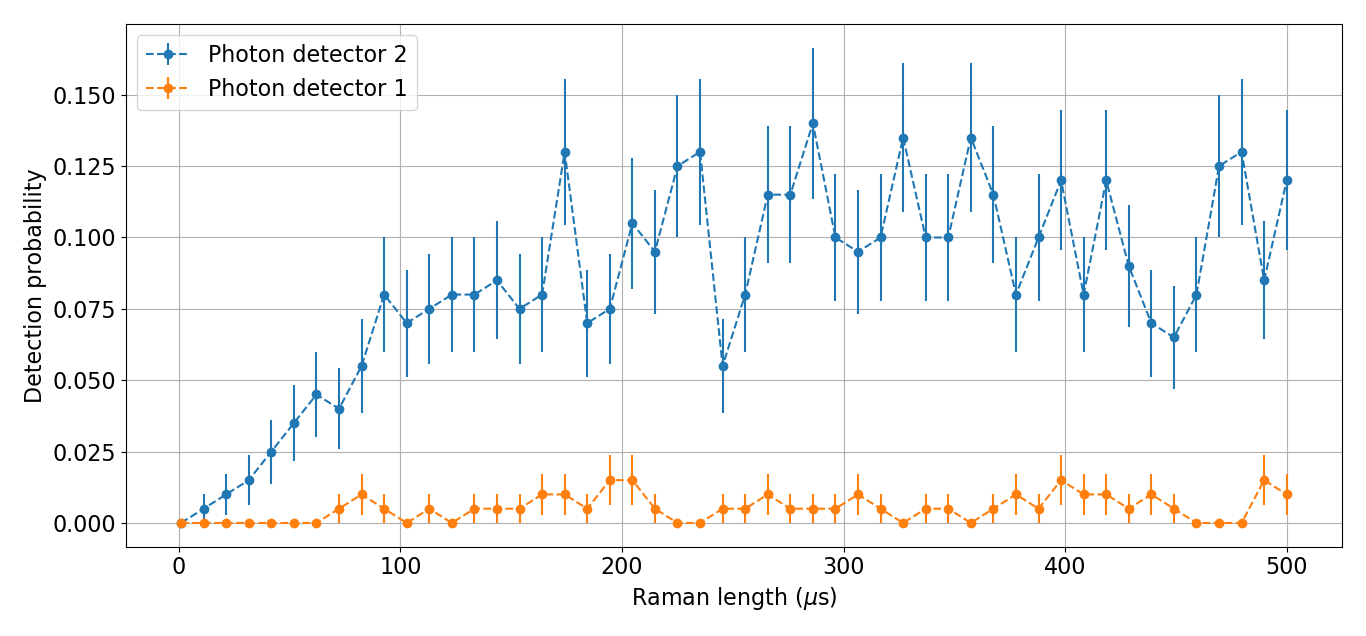
\includegraphics[width=\textwidth]{img/photonefficency_witherror}
\caption{Generated photon efficency}
\end{figure}

\begin{figure}[H]
\centering
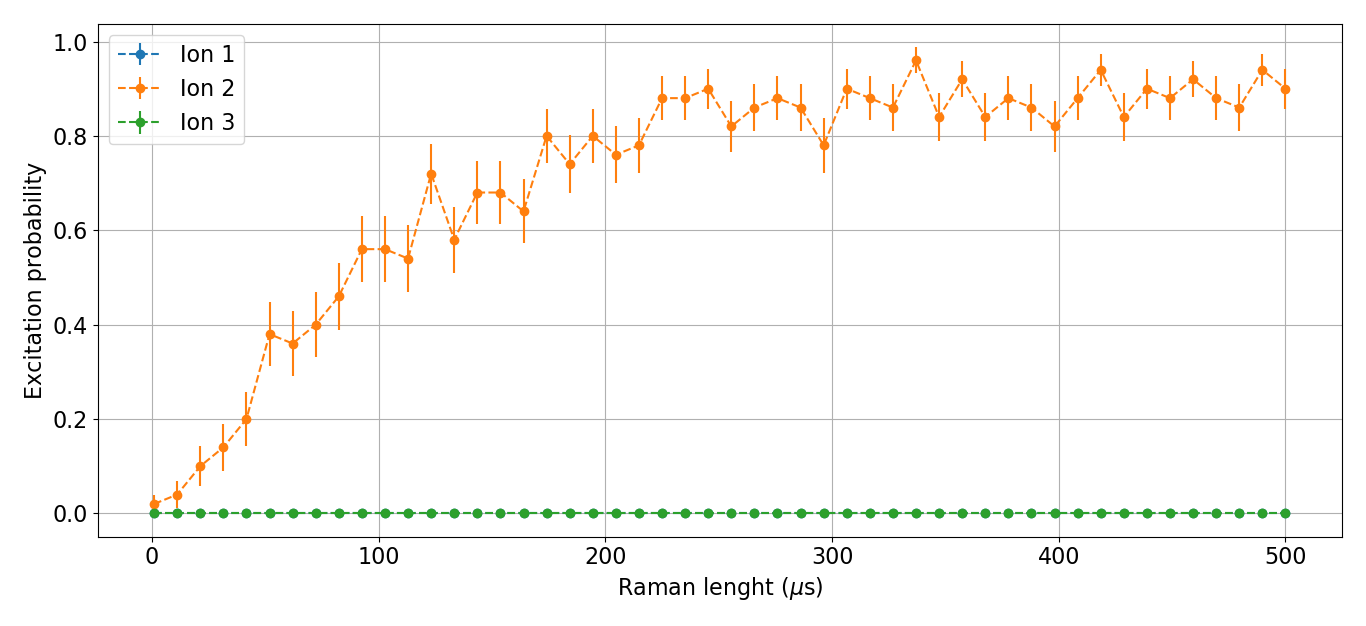
\includegraphics[width=\textwidth]{img/ramanlength_witherrors}
\caption{Excitation of ion while emitting photon}
\end{figure}

- g2 plot?
\section{Final properties summary}
